% Paquets généraux
\documentclass[a4paper,12pt,titlepage]{article}
\usepackage[T1]{fontenc}
\usepackage[utf8]{inputenc}
\usepackage[french]{babel}
\usepackage[gen]{eurosym}
%\usepackage[dvips]{graphicx}
\usepackage{fancyhdr}
\usepackage{pdfpages} 
\usepackage{multido}
\usepackage{moreverb}
\usepackage{hyperref}
%\usepackage{textcomp}
\usepackage{verbatim}
\usepackage{moreverb}
\usepackage{listings}
\usepackage{minted}
\usepackage{eso-pic}
\usepackage{enumitem}
\usepackage{comment}
\usepackage{boxedminipage}
\usepackage[french,onelanguage, boxruled,linesnumbered]{algorithm2e}


\newcommand{\auteurun}{Juliette Genzmer}
\newcommand{\auteurdeux}{Willie Robert}
\newcommand{\auteurtrois}{Renaud Costadoat}
\newcommand{\institute}{Lycée Dorian}
\newtheorem{solution}{Solution}


\newcommand{\nom}{Porte conteneur}
\newcommand{\sequence}{03}
\newcommand{\num}{04}
\newcommand{\type}{TD}
\newcommand{\descrip}{Résolution d'un problème en utilisant des méthodes algorithmiques}
\newcommand{\competences}{Alt-C3: Concevoir un algorithme répondant à un problème précisément posé}

\usepackage{color}
\usepackage{xcolor}
\usepackage{colortbl}
\usepackage{helvet}
\renewcommand{\familydefault}{\sfdefault}
\usepackage{amsfonts}
\usepackage{amsmath}
%\usepackage{xspace}
\usepackage{varioref}
\usepackage{tabularx}
%\usepackage{floatflt}
\usepackage{graphics}
\usepackage{wrapfig}
\usepackage{textcomp}
\usepackage{tikz}
\usepackage{wrapfig}
\usepackage{gensymb}
\usepackage{ifthen}
\usepackage{cancel}
\usepackage{etoolbox}
\usepackage{multirow}
%\usepackage{boxedminipage}
\definecolor{gris25}{gray}{0.75}
\definecolor{bleu}{RGB}{18,33,98}
\definecolor{bleuf}{RGB}{42,94,171}
\definecolor{bleuc}{RGB}{231,239,247}
\definecolor{rougef}{RGB}{185,18,27}
\definecolor{rougec}{RGB}{255,188,204}%255,230,231
\definecolor{vertf}{RGB}{103,126,82}
\definecolor{vertc}{RGB}{220,255,191}
\definecolor{forestgreen}{rgb}{0.13,0.54,0.13}
\definecolor{blcr}{rgb}{0.59,0.69,0.84}
\definecolor{blfr}{rgb}{0.32,0.51,0.75}
\definecolor{orfr}{rgb}{0.90,0.42,0.15}
\definecolor{orcr}{rgb}{0.90,0.65,0.50}
\definecolor{orangef}{rgb}{0.659,0.269,0.072}
\definecolor{orange}{rgb}{0.58,0.35,0.063}
\definecolor{orangec}{rgb}{0.43,0.32,0.25}
\definecolor{rcorrect}{rgb}{0.6,0,0}
\definecolor{sequence}{rgb}{0.75,0.75,0.75}
\definecolor{competences}{rgb}{0.61,0.73,0.35}
\definecolor{grisf}{HTML}{222222}
\definecolor{grisc}{HTML}{636363}
\definecolor{normal}{HTML}{4087c4}
\definecolor{info}{HTML}{5bc0de}
\definecolor{success}{RGB}{92,184,92}
\definecolor{warning}{RGB}{240,173,78}
\definecolor{danger}{RGB}{217,83,79}
\hypersetup{                    % parametrage des hyperliens
    colorlinks=true,                % colorise les liens
    breaklinks=true,                % permet les retours à la ligne pour les liens trop longs
    urlcolor= blfr,                 % couleur des hyperliens
    linkcolor= orange,                % couleur des liens internes aux documents (index, figures, tableaux, equations,...)
    citecolor= forestgreen                % couleur des liens vers les references bibliographiques
    }

% Mise en page
\pagestyle{fancy}

\setlength{\hoffset}{-18pt}

\setlength{\oddsidemargin}{0pt} 	% Marge gauche sur pages impaires
\setlength{\evensidemargin}{0pt} 	% Marge gauche sur pages paires
\setlength{\marginparwidth}{00pt} 	% Largeur de note dans la marge
\setlength{\headwidth}{481pt} 	 	% Largeur de la zone de tête (17cm)
\setlength{\textwidth}{481pt} 	 	% Largeur de la zone de texte (17cm)
\setlength{\voffset}{-18pt} 		% Bon pour DOS
\setlength{\marginparsep}{7pt}	 	% Séparation de la marge
\setlength{\topmargin}{-30pt} 		% Pas de marge en haut
\setlength{\headheight}{55pt} 		% Haut de page
\setlength{\headsep}{20pt} 		% Entre le haut de page et le texte
\setlength{\footskip}{30pt} 		% Bas de page + séparation
\setlength{\textheight}{700pt} 		% Hauteur de l'icone zone de texte (25cm)
\setlength\fboxrule{1 pt}
\renewcommand{\baselinestretch}{1}
\setcounter{tocdepth}{1}
\newcommand{\cadre}[2]
{\fbox{
  \begin{minipage}{#1\linewidth}
   \begin{center}
    #2\\
   \end{center}
  \end{minipage}
 }
}

\newcounter{num_quest} \setcounter{num_quest}{0}
\newcounter{num_rep} \setcounter{num_rep}{0}
\newcounter{num_cor} \setcounter{num_cor}{0}

\newcommand{\question}[1]{\refstepcounter{num_quest}\par
~\ \\ \parbox[t][][t]{0.15\linewidth}{\textbf{Question \arabic{num_quest}}}\parbox[t][][t]{0.85\linewidth}{#1\label{q\the\value{num_quest}}}\par\par
}



\newcommand{\reponse}[0]{\refstepcounter{num_rep}\par
~\ \\ \parbox[t][][t]{0.15\linewidth}{\textbf{Question \arabic{num_rep}}}}

\newcommand{\cor}
{\refstepcounter{num_cor}
\noindent
\rule{\linewidth}{.5pt}
\textbf{Question \arabic{num_cor}:} \\
}



% En tête et pied de page
\lhead{\nom}
\rhead{
\includegraphics[width=2cm]{../../../img/logo}}
\lfoot{David Aubert, Renaud Costadoat}
\rfoot{Page \thepage}
\cfoot{}

\newlength{\RoundedBoxWidth}
\newsavebox{\GrayRoundedBox}
\newenvironment{GrayBox}[1][\dimexpr\textwidth-4.5ex]%
   {\setlength{\RoundedBoxWidth}{\dimexpr#1}
    \begin{lrbox}{\GrayRoundedBox}
       \begin{minipage}{\RoundedBoxWidth}}%
   {   \end{minipage}
    \end{lrbox}
    \begin{center}
    \begin{tikzpicture}%
       \draw node[draw=bleuf,fill=bleuc,rounded corners,%
             inner sep=2ex,text width=\RoundedBoxWidth]%
             {\usebox{\GrayRoundedBox}};
    \end{tikzpicture}
    \end{center}}

\fancypagestyle{correction}{%
  \fancyhf{}
  \lhead{\colorbox{danger}{\begin{minipage}{0.65\paperwidth} \textcolor{white}{\textbf{Correction}} \end{minipage}} }
  \rhead{
\includegraphics[width=2cm]{../../../img/logo}}
  \lfoot{Juliette Genzmer, Willie Robert, Renaud Costadoat}
  \rfoot{\colorbox{danger}{\begin{minipage}{0.3\paperwidth} \begin{flushright}\textcolor{white}{\textbf{Correction}}\end{flushright} \end{minipage}} }}

\renewcommand{\footrulewidth}{0.4pt}


\newcommand{\BackgroundPic}{%
\put(0,0){%
\parbox[b][\paperheight]{\paperwidth}{%
\vfill
\begin{center}
\hspace{0.5cm}\vspace{0.5cm}

\includegraphics[width=\paperwidth,height=\paperheight,%
keepaspectratio]{../../../img/fond5}%
\end{center}
\vfill
}}}

\newcommand{\goforum}{
\begin{figure}[ht!]
\begin{center}
 
\includegraphics[width=0.7\linewidth]{../../../img/go_forum}
\end{center}
\label{go_forum}
\caption{J'pète les plombs}
\end{figure}}

\newcommand{\BackgroundPicdeux}{%
\put(25,-30){%
\parbox[b][\paperheight]{\paperwidth}{%
\vfill
\begin{center}

\includegraphics[width=\paperwidth,height=\paperheight,%
keepaspectratio]{../../../img/fond6}%
\end{center}
\vfill
}}}

\setenumerate[1]{align=left,label=\arabic*}
\setenumerate[2]{before=\stepcounter{enumi},label*=.\arabic*,leftmargin=1.2em,align=left}

\begin{document}


\pagestyle{fancy}

\AddToShipoutPicture{\BackgroundPicdeux}

\begin{center}
{\Large\bf {\type} \no {\numero} -- \descrip}
\end{center}

\SetKw{KwFrom}{de} 

\begin{boxedminipage}{.9\textwidth} 
\begin{itemize}
 \item Faire tous les exercices dans un fichier {NomPrenom.py} à sauvegarder,
 \item mettre en commentaire l'exercice et la question traités (ex: \# Exercice 1),
 \item ne pas oublier pas de commenter ce qui est fait dans votre code (ex: \# Je crée une fonction pour calculer la racine d'un nombre),
 \item il est possible de demander un déblocage pour une question, mais celle-ci sera notée 0,
 \item il faut vérifier avant de partir que le code peut s'exécuter et qu'il affiche les résultats que vous attendez. Les lignes de code qui doivent s'exécuter sont décommentées.
\end{itemize}
\end{boxedminipage}

\section{Introduction}

Le plan du métro parisien a beaucoup évolué au cours du XXème siècle.

~\

\hspace{-0.5cm}
\begin{tabular}{|m{0.3\linewidth}|m{0.3\linewidth}|m{0.3\linewidth}|}
\hline
1903 & 1914 & 1920\\
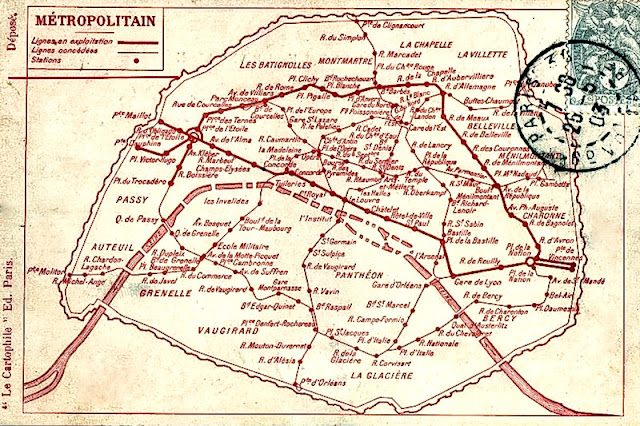
\includegraphics[width=\linewidth]{img/1903}&
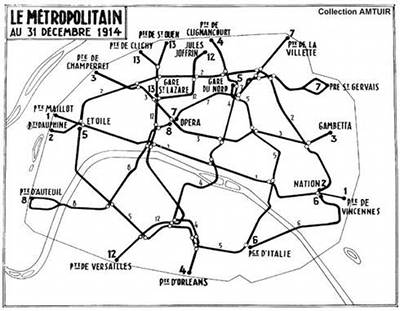
\includegraphics[width=\linewidth]{img/1914}&
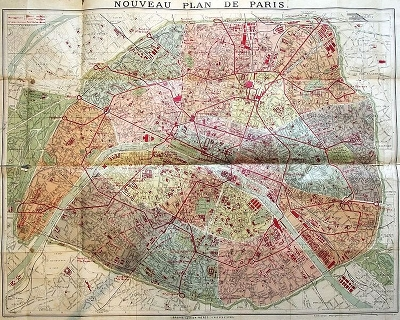
\includegraphics[width=\linewidth]{img/1920}\\
\hline
1930 & 1939 & 1950\\
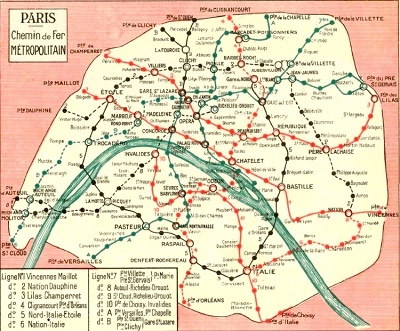
\includegraphics[width=\linewidth]{img/1930}&
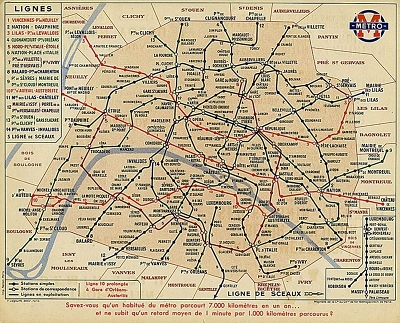
\includegraphics[width=\linewidth]{img/1939}&
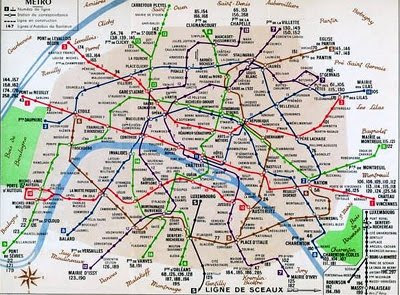
\includegraphics[width=\linewidth]{img/1950}\\
\hline
1963 & 1967 & 1970\\
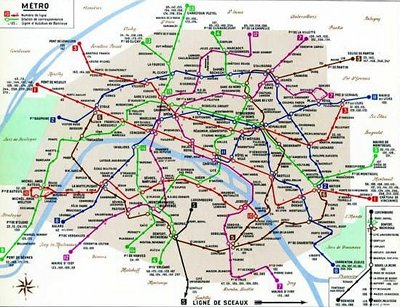
\includegraphics[width=\linewidth]{img/1963}&
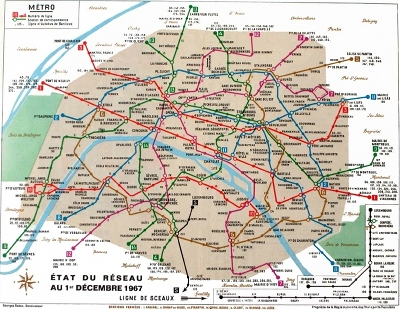
\includegraphics[width=\linewidth]{img/1967}&
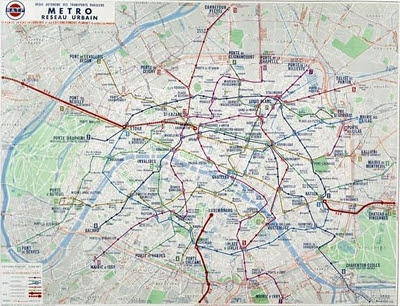
\includegraphics[width=\linewidth]{img/1970}\\
\hline
\end{tabular}

\hspace{-0.5cm}
\begin{tabular}{|m{0.3\linewidth}|m{0.3\linewidth}|m{0.3\linewidth}|}
\hline
1978 & 1980 & 1991\\
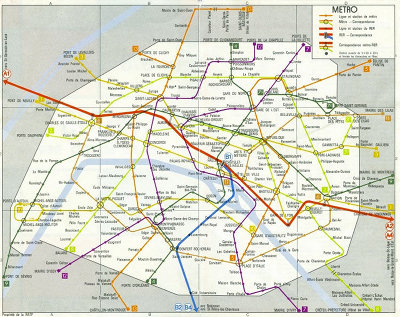
\includegraphics[width=\linewidth]{img/1978}&
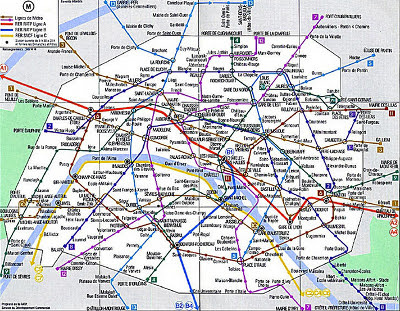
\includegraphics[width=\linewidth]{img/1980}&
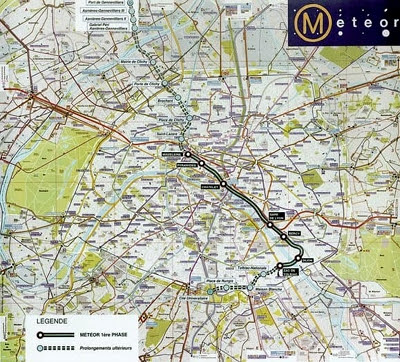
\includegraphics[width=\linewidth]{img/1991}\\
\hline
1999& 2000 & 2015\\
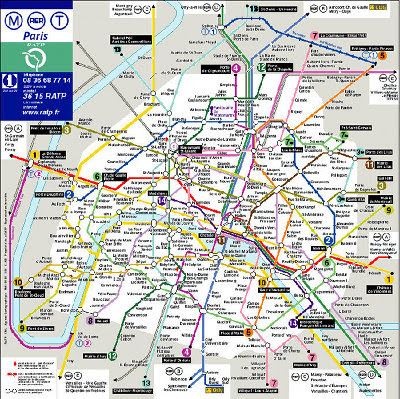
\includegraphics[width=\linewidth]{img/1999}&
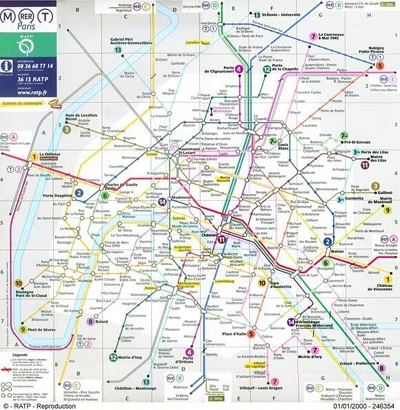
\includegraphics[width=\linewidth]{img/2000}&
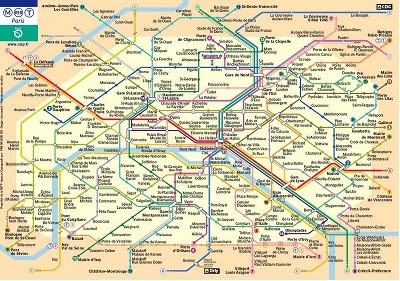
\includegraphics[width=\linewidth]{img/2015}\\
\hline
\end{tabular}

~\

L'objectif de cette épreuve est de tracer le parcours d'une ligne de métro sur une carte à partir des données GPS des stations de métro de Paris.

Les données seront récupérées sur les deux fichiers csv dont le séparateur de colonne est le symbole ';' : \verb?metro-paris-init.csv? et \verb?metro-paris.csv?. Ces fichiers sont disponibles dans le répertoire \og/home/eleve/Ressources/PTSI/\fg, ils ne doivent pas être déplacés mais ouverts directement depuis leur emplacement initial.

Les données ont été extraites d'une base contenant l'ensemble des stations de métro en France. Elle est disponible en suivant le lien suivant:\\
\href{https://www.data.gouv.fr/fr/datasets/lignes-et-stations-de-metro-en-france/}{https://www.data.gouv.fr/fr/datasets/lignes-et-stations-de-metro-en-france/}

\section{Affichage de la carte}

Afin de visualiser le tracé du métro sur une carte de Paris, nous allons grâce au code suivant importer une carte et l'afficher. La commande \verb?plt.show()? trace la courbe et réinitialise les tracé, il faut, pour que la carte puisse être affichée dans la suite, la recharger avec la commande \verb?plt.imshow(...)?, c'est pour cela que la ligne apparaît deux fois dans le code.

\begin{minted}{python}
import matplotlib.pyplot as plt
import matplotlib.image as mpimg
import numpy as np
img=mpimg.imread('paris-map_b.png')
imgplot = plt.imshow(img, interpolation='none', aspect='auto')
plt.axis('equal')
plt.show()
imgplot = plt.imshow(img, interpolation='none', aspect='auto')
\end{minted}

\question{\textbf{Recopier} le code ci-dessus et \textbf{l'exécuter} afin d'afficher la carte de Paris.}

~\

Le fichier \verb?metro-paris-init.csv? contient les coordonnées de 4 stations \og cardinales \fg du métro parisien qui sont situées à l'ouest (\textit{La Défense (Grande Arche)}), au nord (\textit{Porte de Clignancourt}), à l'est (\textit{Château de Vincennes}) et au sud (\textit{Porte d'Orléans}).

La positon de ces stations va permettre d'effectuer le calage entre les coordonnées GPS des stations et un équivalent pixels sur la carte image en png.

Pour cela, il faut commencer par lire le fichier \verb?metro-paris-init.csv? et à partir de celui-ci générer une liste \verb?stations_init? contenant la liste des 4 stations \og cardinales \fg, avec pour chaque station, son nom et une liste contenant sa latitude et sa longitude.

Ainsi, le premier des 4 éléments de la liste \verb?stations_init? est alors:\\
\verb?['"La Défense (Grande Arche)"', [48.89181786551305, 2.237988183098827]]?.

\question{\textbf{Proposer} un code permettant de lire le fichier \texttt{metro-paris-init.csv} et de générer la liste \texttt{stations\_init}.}

~\

Le code suivant est fourni dans le fichier \verb?code_fourni.py? disponible dans le dossier \og/home/eleve/Ressources/PTSI/\fg vous pouvez le copier/coller dans votre script.

\begin{minted}{python}
# CODE FOURNI

# Coordonnées des stations en équivalent pixel sur la carte
coord_carte=[[197,187],[818,136.5],[1376.6,607.3],[706.6,792.2]]

# Calcul de l'échelle de la carte
rayon_terre=6361
distance_ns=rayon_terre*np.tan(np.pi*(stations_init[1][1][0]\
	-stations_init[0][1][0])/180.)
distance_eo=rayon_terre*np.tan(np.pi*(stations_init[1][1][1]\
	-stations_init[0][1][1])/180.)
echelle=[[distance_ns/(coord_carte[1][1]-coord_carte[0][1])],\
	[distance_eo/(coord_carte[1][0]-coord_carte[0][0])]]

# Fonction pour convertir les coordonnées GPS en équivalent pixel sur la carte image
def gps_to_map(coord_station):
    coord_px_x=rayon_terre*np.tan(np.pi*(coord_station[1]\
    	-stations_init[0][1][1])/180.)/echelle[1]+coord_carte[0][0]
    coord_px_y=rayon_terre*np.tan(np.pi*(coord_station[0]\
    	-stations_init[0][1][0])/180.)/echelle[0]+coord_carte[0][1]
    return coord_px_x,coord_px_y

# Tracé des stations sur la carte
for idx,station in enumerate(stations_init):
    coord_px_x,coord_px_y=gps_to_map(station[1])
    plt.scatter(coord_px_x,coord_px_y,s=30,c ='red')

# Tracé de la figure
plt.axis('equal')
plt.show()
imgplot = plt.imshow(img, interpolation='none', aspect='auto')

\end{minted}

\question{\textbf{Copier/coller} le code fourni et l'exécuter. Si votre code fonctionne bien, la carte de Paris doit apparaître avec 4 points rouges au niveau des 4 stations \og cardinales \fg.}

~\

Maintenant que la carte a été calée et que la fonction \verb?gps_to_map(coord_station)? a été définie, il est possible de placer les stations sur la carte.

\question{En reprenant les codes des questions 2 et 3. \textbf{Proposer} un code permettant de générer la liste \verb?stations? des stations de la ligne 1, au même format que la liste \texttt{stations\_init} et \textbf{d'afficher} sur la carte l'ensemble des points correspondants à ces stations.}

\question{\textbf{Modifier} le code de la question précédente afin de tracer la ligne reliant chacune des stations dans l'ordre dans lequel elle apparaît dans la liste. On rappelle que la fonction \verb?plt.plot(x,y)? admet en entrée deux listes \verb?x? et \verb?y? contenant respectivement l'ensemble des coordonnées en $x$ et en $y$ de tous les points à relier.}

\begin{figure}[ht!]
\begin{center}
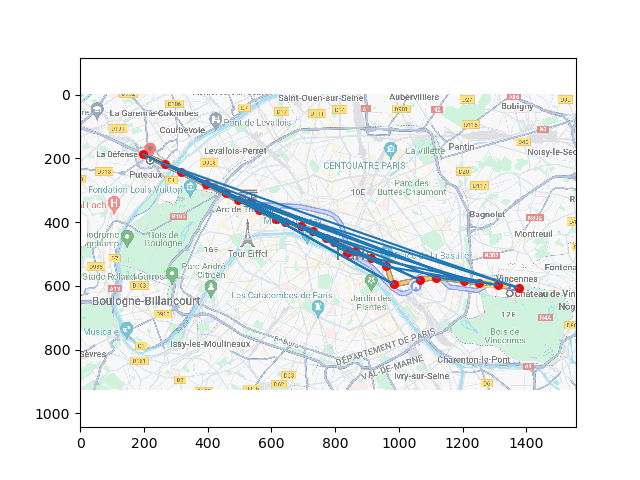
\includegraphics[width=0.5\linewidth]{img/fig02}
\end{center}
\caption{\label{fig01} Premier tracé du parcours de la ligne 1}
\end{figure}

La figure \ref{fig01} montre le tracé de la ligne 1 obtenu grâce à la question 5. Le résultat n'est pas très probant.

\section{Calcul de distance}

Dans cette partie, l'objectif va être de déterminer la distance en km entre deux points $A[lati_A,long_A]$ et $B[lati_B,long_B]$ définis par leurs coordonnées GPS.

Pour cela on utilise la formule suivante:
\begin{center}
$distance=arccos(sin(\varphi_1)\times sin(\varphi_2)+cos(\varphi_1)\times cos(\varphi_2)
\times cos(\lambda))\times R$
\end{center}

Avec:
\begin{center}
$\left\{\begin{array}{l}
\varphi_1=lati_A*\frac{\pi}{180}\\
\varphi_2=lati_B*\frac{\pi}{180}\\
\lambda=(long_B-long_A)*\frac{\pi}{180}\\
R: Rayon\ de\ la\ terre
\end{array}\right.$
\end{center}

\question{\textbf{Coder} la fonction \texttt{distance(stationA,stationB)} qui renvoie la distance entre deux stations. Les stations en entrée de la fonction seront définies comme l'exemple suivant :}
\begin{center}
\verb?stationA=['"La Défense (Grande Arche)"',[48.891817865513, 2.2379881830988]]?
\end{center}

Ainsi, la commande \verb?print(distance(stations_init[0],stations_init[2]))? renvoie \verb?15.704007162540035?.

\section{Algorithme glouton}

Afin de respecter l'ordre des stations d'une ligne durant le parcours, on va supposer que la station suivante est la plus proche. On verra que, selon les lignes, ce n'est pas toujours le cas.

Pour cela, nous allons générer une liste \verb?liste_station_ordre? grâce  à un algorithme glouton. Au départ, celle-ci ne contient que \verb?stations[0]?.

L'algorithme à utiliser est le suivant:
\begin{itemize}
 \item Partir de la dernière station de la liste \verb?liste_station_ordre?,
 \item Chercher la station de la ligne 1 la plus proche (dont la distance est la plus petite) ET qui n'est pas déjà dans \verb?liste_station_ordre?,
 \item Ajouter cette nouvelle station à \verb?liste_station_ordre?,
 \item Recommencer à la première étape jusqu'à avoir récupéré toutes les stations de la ligne 1. 
\end{itemize}

\question{\textbf{Coder} l'algorithme précédent afin de générer la liste \texttt{liste\_station\_ordre} puis parcourir cette liste afin de \textbf{tracer} les points et le parcours de la ligne sur la carte comme pour les questions 4 et 5.}

~\

Normalement, cette fois-ci le tracé est beaucoup plus probant.

\question{\textbf{Générer} et \textbf{afficher} la liste des distances parcourues cumulées, en mètre, au fur et à mesure du parcours de la ligne 1.}

~\

On obtient le résultat suivant :
\begin{center}
\verb?distances=[0, 382, 1117, 1605, 2076, 2647, 3500, 4582, 5285,...]?
\end{center}

\newpage

\section{Dichotomie}

\verb?L=[1,3,5,7,10,13]?

\question{Soit la liste \verb?L? coder une fonction \texttt{dichotomie(L,a)} qui renvoie l'index d'une valeur dans la liste si celle-ci existe et \verb?False? si la valeur n'est pas dans la liste.}

~\

Ex: \verb?dichotomie(L,3)? renvoie \verb?1? et \verb?dichotomie(L,4)? renvoie \verb?False?.

\question{Soit la liste \verb?L? coder une fonction \texttt{dichotomie\_interval} qui renvoie l'index d'une valeur dans la liste si celle-ci existe et les index des valeurs juste inférieure et juste supérieure si la valeur n'est pas dans la liste.}

~\

Ex: \verb?dichotomie_interval(L,3)? renvoie \verb?1? et \verb?dichotomie_interval(L,4)? renvoie \verb?(1,2)?

\question{Utiliser cette fonction pour déterminer combien de stations doivent être parcourues pour faire 10km sur la ligne 1.}

\section{Tracé de ligne}

\question{\textbf{Coder} une fonction \texttt{trace\_ligne(numero)} qui prend en entrée un numéro de ligne de métro et qui retourne le tracé de la ligne sur la carte. \textbf{Tester} la fonction avec la commande \texttt{trace\_ligne(4)
}.}


\begin{center}
\Large{FIN}
\end{center}


\ifdef{\public}{Remarque : La suite du document peut et \textbf{doit} servir de brouillon.

~\

\feuilleDR{10}

\end{document}}{\cleardoublepage\pagestyle{correction}}


\begin{center}
\Large{Correction}
\end{center}

\reponse{}

\begin{minted}{python}
import matplotlib.pyplot as plt
import matplotlib.image as mpimg
import numpy as np

img=mpimg.imread('paris-map_b.png')
imgplot = plt.imshow(img, interpolation='none', aspect='auto')
plt.axis('equal')
plt.show()
imgplot = plt.imshow(img, interpolation='none', aspect='auto')
\end{minted}

\reponse{}

\begin{minted}{python}
file=open('metro-paris-init.csv','r')
lignes=file.read().split('\n')
file.close()

stations_init=[]

for ligne in lignes[1:-1]:
    data=ligne.split(';')
    lati=float(data[4])
    long=float(data[3])
    stations_init.append([data[2],[lati,long]])

print(stations_init)
\end{minted}

\reponse{}

\begin{minted}{python}
# Coordonnées des stations en équivalent pixel sur la carte
coord_carte=[[197,187],[818,136.5],[1376.6,607.3],[706.6,792.2]]

# Calcul de l'échelle de la carte
rayon_terre=6361
distance_ns=rayon_terre*np.tan(np.pi*(stations_init[1][1][0]\
	-stations_init[0][1][0])/180.)
distance_eo=rayon_terre*np.tan(np.pi*(stations_init[1][1][1]\
	-stations_init[0][1][1])/180.)
echelle=[[distance_ns/(coord_carte[1][1]-coord_carte[0][1])],\
	[distance_eo/(coord_carte[1][0]-coord_carte[0][0])]]

# Fonction pour convertir les coordonnées GPS en équivalent pixel sur la carte image
def gps_to_map(coord_station):
    coord_px_x=rayon_terre*np.tan(np.pi*(coord_station[1]\
    	-stations_init[0][1][1])/180.)/echelle[1]+coord_carte[0][0]
    coord_px_y=rayon_terre*np.tan(np.pi*(coord_station[0]\
    	-stations_init[0][1][0])/180.)/echelle[0]+coord_carte[0][1]
    return coord_px_x,coord_px_y

# Tracé des stations sur la carte
for idx,station in enumerate(stations_init):
    coord_px_x,coord_px_y=gps_to_map(station[1])
    plt.scatter(coord_px_x,coord_px_y,s=30,c ='red')

# Tracé de la figure
plt.axis('equal')
plt.show()
imgplot = plt.imshow(img, interpolation='none', aspect='auto')
\end{minted}

\reponse{}

\begin{minted}{python}
file=open('metro-paris.csv','r')
lignes=file.read().split('\n')
file.close()

stations=[]
x=[]
y=[]
for ligne in lignes[1:-1]:
    data=ligne.split(';')
    lati=float(data[4])
    long=float(data[3])
    if data[1]=='1':
        stations.append([data[2],[lati,long]])
        coord_px_x,coord_px_y=gps_to_map([lati,long])
        plt.scatter(coord_px_x,coord_px_y,s=30,c ='red')

plt.axis('equal')
plt.savefig('img/fig02.png')
plt.show()
imgplot = plt.imshow(img, interpolation='none', aspect='auto')
\end{minted}

\reponse{}

\begin{minted}{python}
file=open('metro-paris.csv','r')
lignes=file.read().split('\n')
file.close()

stations=[]
x=[]
y=[]
for ligne in lignes[1:-1]:
    data=ligne.split(';')
    lati=float(data[4])
    long=float(data[3])
    if data[1]=='1':
        stations.append([data[2],[lati,long]])
        coord_px_x,coord_px_y=gps_to_map([lati,long])
        plt.scatter(coord_px_x,coord_px_y,s=30,c ='red')
        x.append(coord_px_x)
        y.append(coord_px_y)

plt.plot(x,y)
plt.axis('equal')
plt.savefig('img/fig02.png')
plt.show()
imgplot = plt.imshow(img, interpolation='none', aspect='auto')
\end{minted}

\reponse{}

\begin{minted}{python}
def distance(stationA,stationB):
    phi1=stationA[1][0]*np.pi/180
    phi2=stationB[1][0]*np.pi/180
    deltalambda=(stationB[1][1]-stationA[1][1])*np.pi/180
    return np.arccos(np.sin(phi1)*np.sin(phi2)+np.cos(phi1)*np.cos(phi2)*np.cos(deltalambda))*rayon_terre

print(distance(stations_init[0],stations_init[2]))
print(distance(stations_init[1],stations_init[3]))
\end{minted}

\reponse{}

\begin{minted}{python}
liste_station_ordre=[stations[0]]
for idx_sta in range(len(stations)-1):
    min=20
    for station in stations:
        if station not in liste_station_ordre and distance(liste_station_ordre[-1],station)<min:
            min=distance(liste_station_ordre[-1],station)
            next_station=station
    liste_station_ordre.append(next_station)

x=[]
y=[]
for station in liste_station_ordre:
    coord_px_x,coord_px_y=gps_to_map(station[1])
    plt.scatter(coord_px_x,coord_px_y,s=30,c ='red')
    x.append(coord_px_x)
    y.append(coord_px_y)

plt.plot(x,y)


# Tracé de la figure
plt.axis('equal')
plt.savefig('img/fig03.png')
plt.show()
imgplot = plt.imshow(img, interpolation='none', aspect='auto')
\end{minted}

\reponse{}

\begin{minted}{python}
liste_station_ordre=[stations[0]]
distances=[0]
for idx_sta in range(len(stations)-1):
    min=20
    for station in stations:
        if station not in liste_station_ordre and distance(liste_station_ordre[-1],station)<min:
            min=distance(liste_station_ordre[-1],station)
            next_station=station
    distances.append(int(1000*min+distances[-1]))
    liste_station_ordre.append(next_station)

print(distances)
\end{minted}

\reponse{}

\begin{minted}{python}
L=[1,3,5,7,10,13]

def dichotomie(L, a):
    debut = 0
    fin = len(L) - 1
    while debut <= fin:
        m = (debut+fin) // 2
        if L[m] == a:
            return m
        elif L[m] < a:
            debut = m+1
        else:
            fin = m-1
    return False

print(dichotomie(L, 12))
\end{minted}

\reponse{}

\begin{minted}{python}
def dichotomie_inter(L, a):
    debut = 0
    fin = len(L) - 1
    while debut+1 < fin:
        m = (debut+fin) // 2
        if L[m] == a:
            return m
        elif L[m] < a:
            debut = m
        else:
            fin = m
    return (debut,fin)

print(dichotomie_inter(L, 12))
\end{minted}

\reponse{}

\begin{minted}{python}
print(dichotomie_inter(distances, 10000))
\end{minted}

\reponse{}

\begin{minted}{python}
def trace_ligne(numero):
    file=open('metro-paris.csv','r')
    lignes=file.read().split('\n')
    file.close()

    stations=[]

    x=[]
    y=[]
    for ligne in lignes[1:-1]:
        data=ligne.split(';')
        lati=float(data[4])
        long=float(data[3])
        if data[1]==str(numero):
            stations.append([data[2],[lati,long]])
            coord_px_x,coord_px_y=gps_to_map([lati,long])
            plt.scatter(coord_px_x,coord_px_y,s=30,c ='red')
            x.append(coord_px_x)
            y.append(coord_px_y)

    liste_station_ordre=[stations[0]]
    for idx_sta in range(len(stations)-1):
        min=1
        for station in stations:
            if station not in liste_station_ordre and distance(liste_station_ordre[-1],station)<min:
                min=distance(liste_station_ordre[-1],station)
                next_station=station
        liste_station_ordre.append(next_station)

    x=[]
    y=[]
    for station in liste_station_ordre:
        coord_px_x,coord_px_y=gps_to_map(station[1])
        plt.scatter(coord_px_x,coord_px_y,s=30,c ='red')
        x.append(coord_px_x)
        y.append(coord_px_y)

    plt.plot(x,y)


    # Tracé de la figure
    plt.axis('equal')
    plt.savefig('img/fig04.png')
    plt.show()
    imgplot = plt.imshow(img, interpolation='none', aspect='auto')

trace_ligne(4)
\end{minted}

\end{document}
